\chapter{Описание существующих решений}

В данном разделе представлено краткое описание существующих методов обработки текстов на каждом этапе работы вопросно-ответной системы.

\section{Этап анализа вопроса}

\subsection{Символьные шаблоны вопросов}
Одним из способом определить тэг или фокус в вопросе является подготовка шаблонов (регулярных выражений) для распознавания распространенного вопросительного оборота~\cite{step1}. В таблице~\ref{tb:oe} приведены некоторые правила, используемые в системе OpenEphyra для английского языка~\cite{step11}:

\begin{table}[h!]
	\begin{center}
		\begin{threeparttable}
			\captionsetup{justification=raggedright,singlelinecheck=off}
			\caption{\label{tb:oe}Символьные шаблоны вопросов из системы OpenEphyra}
			\begin{tabular}{|c|c|}
				\hline
				\textbf{Семантический тэг} & \textbf{Регулярное выражение вопроса} \\ [0.8ex] 
				\hline
				Date → Weekday & (what|which|name) (.* )?(day of (the )?week|weekday)\\
				\hline
				Location → Country & (what|which|name) (.* )?(colony|country|nation)\\
				\hline
				Size → Length & how (deep|far|high|long|tall|wide)\\
				\hline
				Size → Length & (how large in|how many) (foot|inch|.*meter|mile|yard) \\
				\hline
			\end{tabular}
		\end{threeparttable} 
	\end{center}
\end{table}

Недостатки такого подхода следующие.
\begin{enumerate}
	\item Невозможность покрыть большую часть реальных вопросов
	пользователей. Набор вопросов подбирается так, чтобы обработать конкретный
	набор тестовых заданий. Выйти за пределы этого покрытия <<неудобным
	вопросом>> достаточно легко.
	\item Связь между вопросительными словами и семантическими тэгами не так прямолинейна.
	Так,
	слово <<кто>> может подразумевать персону, организацию, страну или народ (например, в вопросе <<Кто захватил Константинополь?>>).
\end{enumerate}

\subsection{Синтаксические шаблоны вопросов}
Для выделения фокуса вопроса следующим шагом после символьных шаблонов стал метод синтаксических шаблонов. Данные шаблоны значительно сложнее символьных, однако могут использоваться в широком круге вопросов. В основе метода лежит предположение, что фокус вопроса часто находится в определённом синтаксическом отношении с вопросительным словом,
может быть не в одном, но набор вариантов этих отношений ограничен~\cite{step1}. 

Сначала выполняется синтаксический разбор предложения, в результате чего получается синтаксическое дерево. Далее это дерево вопроса сравнивается с синтаксическим шаблоном для распознавания фокуса и, в случае совпадения, фокусом считаются члены предложения, соответствующие позиции фокуса в шаблоне.

\subsection{Статистика употребления слов в вопросах}

Это метод автоматического обучения статистической модели для простановки семантического
тэга~\cite{step1}. Для каждого вопроса из обучающей выборки выделяют три <<потока>> признаков:

\begin{itemize}[label=---]
	\item все слова как есть и дополнительные метки к некоторым из них;
	\item метки частей речи слов и порядковые номера слов в предложении;
	\item фокусные слова с гиперонимами, согласно лексическому тезаурусу.
\end{itemize}

После разметки вручную коллекции из вопросов подсчитывается, какие свойства чаще означают каждый семантический тэг. Для этого используется математический аппарат максимизации энтропии. Метод максимума энтропии~\cite{maxentr} является вероятностным классификатором, который основан на принципе максимальной энтропии. По данному принципу распределения вероятности являются равномерными (имеют максимальную энтропию), если нет оснований считать иначе.

Недостатком статистического метода является необходимость создания большой обучающей коллекции вопросов вручную.

\section{Этап информационного поиска}

\subsection{Деление на абзацы}

Наиболее простым способом выделения текстовых фрагментов из набора документов является деление текста на абзацы. Затем выбираются те фрагменты, которые содержат наибольшее количество ключевых слов.

\subsection{Использование окон параграфа}

В вопросно-ответной системе, разработанной в Южном Методистском Университете
США~\cite{step2}, был использован другой способ получения фрагментов документов для последующего извлечения из них ответа.

Например, у нас есть набор ключевых слов {$k1$, $k2$, $k3$, $k4$} и в параграфе текста $k1$ и $k2$ встречаются каждое дважды, тогда как $k3$ --- только один раз, и $k4$ ни разу. Далее вводится понятие окна параграфа --- это фрагмент, содержащий весь текст между ключевым словом с самой низкой позицией в окне и ключевым словом с самой высокой позицией в окне. В данном примере  будет четыре разных окна, определяемых ключевыми словами: [$k1$--соответствие$_1$, $k2$--соответствие$_1$, $k3$], [$k1$--соответствие$_2$, $k2$--соответствие$_1$, $k3$], [$k1$--соответствие$_1$, $k2$--соответствие$_2$, $k3$] и [$k1$--соответствие$_2$, $k2$--соответствие$_2$, $k3$].

Для каждого окна параграфа вычисляются следующие оценки:
\begin{itemize}[label=---]
	\item $Same\_word\_sequence\_score$ содержит количество слов из вопроса, которые распознаются в той же последовательности в текущем окне;
	\item $Distance\_score$ содержит количество слов, разделяющих самые удаленные ключевые слова в окне;
	\item $Missing\_keywords\_score$ содержит количество не попавших в окно ключевых слов. 
\end{itemize}

Далее выполняется сортировка окон параграфов по трем различным показателям:
\begin{itemize}[label=---]
	\item наибольшее значение $Same\_word\_sequence\_score$;
	\item наибольшее значение $Distance\_score$;
	\item наименьшее значение $Missing\_keyword\_score$.
\end{itemize}

\section{Этап извлечения потенциальных ответов}

\subsection{Использование шаблонов}

Для каждого типа ответа составляются шаблоны, с помощью которых в текстовых фрагментах производится поиск и выделение кандидата ответа~\cite{patterns}. Для выбора ответа используется информация о типе ожидаемого ответа, полученная на этапе анализа вопроса, и символьные шаблоны. Шаблоны можно создавать как вручную, так и автоматическими обучаемыми алгоритмами.

\subsection{Использование N-грамм}

N-грамма – это последовательность из N слов, идущих в каком-то тексте подряд. На первом этапе из фрагмента текста извлекаются униграммы, биграммы и триграммы. Каждой из них назначается вес, соответствующий количеству текстовых фрагментов, в которых она нашлась. Далее для каждой N-граммы вес корректируется с учетом типа ожидаемого ответа. После N-граммы ранжируются, выбираются N-граммы с наиболее высокими оценками и конструируется ответ путем объединения перекрывающихся N-грамм~\cite{ngramms}.

\section{Этап валидации ответов}

\subsection{Пересечение множеств слов и/или грамматических отношений}
В данном методе применяется модель мешка слов (англ. \textit{bag of words})~\cite{bag}.
Мера <<подтверждения>> ответа на вопрос вычисляется по формуле~(\ref{eq:21}):
\begin{equation}\label{eq:21}
	 E = \frac{|{Q}\cap{T}|}{|Q|},
\end{equation}

\noindent где $Q$ --- множество слов в вопросе, ~$T$ --- множество слов во фрагменте текста, содержащем потенциальный ответ.

Усложнением является использование не множества слов, а множества
синтаксических отношений, т.е. пар слов, связанных грамматической связью: $R(N1,N2)$~\cite{step4}.

\subsection{Сопоставление сказуемых}

Ответ и фрагмент текста с потенциальным ответом предварительно проходят аннотацию семантическими ролями. В результате слова предложения получают метку либо сказуемого, либо аргумента при каком-то сказуемом. Сравниваются два сказуемых со всеми зависимыми словами: одно сказуемое из вопроса, другое --- из текстового фрагмента. Схожесть двух сказуемых вычисляется как произведение лексической схожести глаголов (например, расстояние по словарю WordNet) и схожести наборов аргументов:
\begin{equation}\label{eq:22}
	Sim_{Pred} = Sim_{Verb} \cdot Sim_{Args}.
\end{equation} 

Схожесть аргументов предиката вопроса $p_q$ и предиката $p_a$ из фрагмента текста вычисляется следующим образом:
\begin{equation}\label{eq:23}
	Sim_{Args}(p_a, p_q) = \frac{\sum\limits_{t_a\in{T_a}}\max\limits_{t_q\in{T_q}}(Sim_{ExpTerm}(t_a, t_q))}
	{|T_q| + |\{t_a\in{T_a}|\max\limits_{t_q\in{T_q}}(Sim_{ExpTerm}(t_a, t_q)) = 0\}|}.
\end{equation}

Мера схожести двух термов вычисляется по формуле (\ref{eq:24}):
\begin{equation}\label{eq:24}
	Sim_{Term}(t_1, t_2) = \frac{|{W1}\cap{W2}|}{|{W1}\cup{W2}|},
\end{equation}

\noindent где $W1$ и $W2$ --- множества контекстных слов из описания значения терма в словаре.

Если в вопросе или фрагменте текста несколько сказуемых, то вычисляется схожесть всех пар.
Наибольшее из полученных чисел и будет мерой подтверждения ответа фрагментом текста~\cite{step4}.

\subsection{Расстояние редактирования для деревьев}

Далее рассматривается задача вычисления схожести деревьев грамматических зависимостей между словами двух предложений: вопросительного и повествовательного~\cite{step4}. Для предложения-кандидата и вопросительного предложения строятся так называемые деревья грамматических зависимостей, отражающие связи между словами, рассматривая их как части речи. Пример дерева для вопросительного предложения приведен на рисунке~\ref{img:tree}~\cite{trees}. 
\begin{figure}[h!]
	\centering
	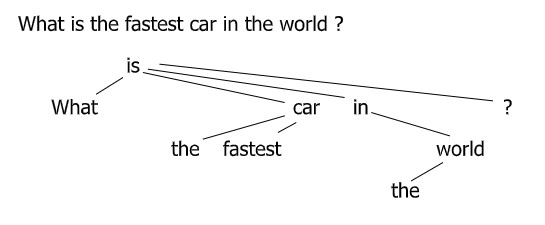
\includegraphics[height=0.2\textheight]{img/tree}
	\caption{Пример дерева грамматических зависимостей для вопроса}
	\label{img:tree}
\end{figure}

В данном методе применяется естественная метрика схожести деревьев: минимальное число операций редактирования, необходимых для трансформации одного графа в другой. Доступные операции редактирования: удаление вершины, вставка, замена. Каждая такая операция $s_i$ имеет некоторый вес $y(s_i)$.

Пусть $S = <s1; s2; …; sk>$ --- последовательность операций, приводящая к трансформации дерева предложения-кандидата на ответ в дерево вопроса. Тогда стоимость этой трансформации есть сумма стоимостей операций.
\begin{equation}\label{eq:25}
	y(S) = \sum{y(s_i)}.
\end{equation}

Последовательность с наименьшей стоимостью операций редактирования вычисляется по формуле~(\ref{eq:26}):
\begin{equation}\label{eq:26}
	\delta(T_p, T_q) = \min\limits_{S}(y(S) | S(T_p) = T_q).
\end{equation}

В итоге выбираются кандидаты с наименьшей оценкой.


